%% The following is a directive for TeXShop to indicate the main file
%%!TEX root = ../../thesis.tex

\chapter{A physical property model for a fractured volume of rock}
\label{ch:phys_prop_model}
\title{A physical property model for a fractured volume of rock}


\section{Introduction}

For electromagnetic methods to be sensitive to a propped, fractured volume of rock, the fractured volume of rock must have physical properties which are distinct from the background, host rock. For EM methods, this means the electrical conductivity, magnetic permeability, or dielectric permittivity of the fractured rock must be distinct. Dielectric permittivity only plays a significant role when the frequency of the source is sufficiently high, in the hundreds of kilohertz to megahertz range, as is used in ground penetrating radar. Over the length-scales which we wish to work, attenuation of the EM signals due to skin depth effects make GPR impractical, thus work in the quasi-static regime of Maxwell's equations and concern ourselves only with magnetic permeability and electrical conductivity. The materials traditionally used as proppant, typically sand and ceramics, tend to have similar physical properties to the reservoir that they are being pumped into, making it difficult to detect them on the scale of the reservoir. However, if the proppant were made electrically conductive or magnetically permeable, for instance by coating it with graphite or including magnetite particles, it may create a sufficient physical property contrast that can be imaged using EM.

Using additives as to make a hydraulic fracture a geophysical target is not a new idea. \cite{Byerlee1976} suggested using magnetic particles and a magnetic survey to estimate fracture orientation at distances larger than can be determined by tracers and well logs. To create a fracture with a significant magnetic susceptibility, they suggest using finely crushed magnetite suspended in the fracturing fluid or iron shot, spherical particles of iron which do not crush easily and have a high magnetic susceptibility. They treat the fracture as a plate with a known magnetic susceptibility and collect measurements before and after the fracture operation; measurements of the horizontal magnetic field inside of the injection borehole are used to indicate the orientation of the fracture and surface measurements are used to estimate the fracture geometry. Using an analytic model for the magnetic response of a circular disc in a uniform inducing field, they demonstrated the potential of this technique for simple analog models of two fields sites: an engineered geothermal project at Los Alamos, where fractures are induced to circulate fluid through a dry geothermal reservoir and a hydraulic fracture operation for a tight-gas reservoir at Rio Blanco.

Similarly, \cite{Bartel1976} suggest using electrically conductive fracturing fluid and measuring electric potentials at the surface in a DC resistivity experiment where one electrode is connected to the injection well and a return electrode is connected to a distant well casing. Potential electrodes are arranged in two concentric rings centered about the injection well with potential differences being measured between electrodes along the same azimuth in the inner and outer rings. Variation in the amplitude of the potential difference with azimuth are used to estimate the orientation of the fracture and to detect asymmetry (e.g. if the fracture extends further one side of the well than the other). Field tests were performed at two sites and demonstrated detectability of fractures in an experiment in the Wattenburg field for fractures at depths of $\sim$2200m depth. The source electrode was connected to the casing and centered at the depth of the induced fracture (see also \cite{Smith1978}).

Since these initial developments in the late 70's, there have been significant improvements in data quality as well as our ability to model and invert electrical and electromagnetic data in 3D. In conjunction, there have been advancements in fracture operations and imaging techniques such as the use of microseismic, tiltmeters, and pressure-transient analysis to characterize hydraulic fracture. As a result, the questions being asked are more detailed. How complex is the fracture? Is is a simple planar fracture or an extensive network (as shown in Figure \ref{fig:frac_complexity}? What is the extent of the ``stimulated reservoir volume,'' the volume of rock in which fractures have been induced and remain open? What is the extent of the propped volume of rock where fractures have been created and remain propped-open with proppant? The large number of fracture operations that have been conducted and monitored with microseismic and tiltmeters in the past few decades indicate that there is significant diversity in fracture complexity and height growth \cite{Cipolla2008}. These factors influence the resultant production of hydrocarbons. Thus, understanding how engineering decisions, such as pumping pressures, proppant particle size and volumes, etc., impact fracture geometry and proppant distribution within those fractures are important for increasing the effectiveness of the hydraulic fracture operations. Microseismic data in particular have contributed significantly to the understanding of fracture complexity and estimating the stimulated reservoir volume \citep{Mayerhofer2010}, however there is significant motivation for improving the characterization of the propped volume of the fractured reservoir. \cite{Hoversten2015} estimate that a 5\% improvement in the characterization of the stimulated reservoir volume for a 1 billion barrel field translates to over 0.5 billion U.S. dollars in net present value over 24 years with oil at US\$50 per barrel.


\begin{figure}
    \begin{center}
    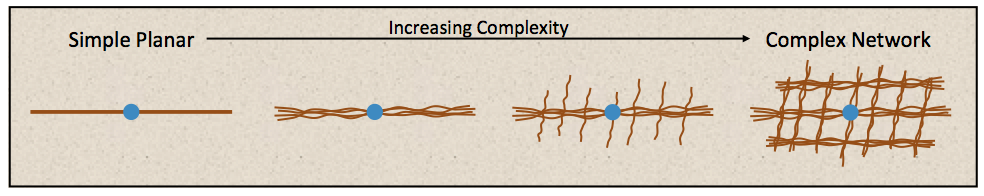
\includegraphics[width=\columnwidth]{figures/phys_prop_model/frac_complexity.png}
    \end{center}
\caption{
    Fracture complexity, from simple planar fractures on the left to complex fracture
    networks on the right. The blue doe is the injection point in a horizontal well. After \cite{Cipolla2008a}.
}
\label{fig:frac_complexity}
\end{figure}


To make the proppant electromagnetically distinct from the host rock, either the magnetic permeability or the electrical conductivity of the proppant could be targeted. \citep{Zawadzki2016} provides an overview of possible magnetic proppants and highlights some practical considerations for the choice of material. For example, the mechanical strength of the particles must be able to withstand the pressure of the closing fracture without crushing and clogging the fracture pathways, the material shouldn’t be toxic or reactive, and the price-point should be reasonable as high volumes are needed. \citep{Zawadzki2016} provide a general classification of material types that could be considered: feedstock material, materials that are mixed with conventional proppant or replace conventional proppant, could include magnetite or steel particles. Both have a significant magnetic permeability, however, magnetite crushes easily, and although steel has significant mechanical strength, it is challenging to manufacture particles that are small enough (typically $< 2$mm in diameter). They also consider ferrofluids, which contain microscopic ferromagnetic particles in suspension, and magnetic nanoparticles. Both are sufficiently small to be used in fractures and remain in suspension so clogging is less of a concern, however the cost of either material is quite significant and steps must be taken to reduce the environmental hazard posed, in particular by nanoparticles, as they tend to be much more reactive than particles of the same material but larger in size \cite{Zawadzki2016}. Continuing advances in nanotechnology has prompted some authors, e.g. \citep{Rahmani2014}, to pursue analysis of the use of magnetic markers for mapping hydraulic fractures using electromagnetic techniques.

Magnetic permeability of common materials tends to vary over an order of magnitude \cite{Telford1990}, while electrical conductivity of common materials can vary over $> 8$ orders of magnitude. Comparatively, there are many more materials that are electrically conductive than there are with a significant magnetic permeability. Materials such as coke breeze, a hardened graphite coating applied to conventional proppants, have been considered by numerous authors, as have a range of manufactured electrically conductive proppants \citep{Pardo2013, Hoversten2015, Weiss2015, Labrecque2016, Hu2018}. For these reasons, we focus on electrically conductive proppants and treat the fractured region of the reservoir as an electrically conductive geophysical target.

Numerical modelling is a critical component for examining the feasibility of detecting a fractured volume of rock with a given electromagnetic survey. To run a simulation, we need to discretize the modelling domain and describe the electrical conductivity model on the simulation mesh. It is important to consider the large range of scales at play when considering fractures. The proppant which fills the fractures is micro-to-millimeters in diameter, and we are aiming to characterize a region of the reservoir which extends hundreds of meters from the injection point at the well, tens to hundreds of meters in height and tens to hundreds of meters along the length of the well-bore. We cannot expect a method to be capable of imaging both such a substantial region of the subsurface while having the resolution on the scale of the proppant particles. Thus, we require a characterization of the bulk impact of the conductive proppant within a fractured volume of rock. How we construct such a bulk physical property model depends on the geometry and complexity of the induced fractures, for instance, different approaches should be considered if the fracture is a simple planar fracture versus a complex fracture network, as depicted in Figure \ref{fig:fracComplexity} (c.f. \cite{Cipolla2008}).

The numerical challenge is that we must capture the effects of the fine scale physical property variations, while being able to model a domain that includes the extent of the fracture. Simply applying a mesh that captures the fine-scale variations will typically lead to a mesh that is too large to work with, and EM surveys lack the resolution to image individual fractures. Thus, we require a method that we can work with computationally and is suitable for the inverse problem.

There are several approaches that may be taken, and the appropriate choice will depend upon both the fracture complexity and the purpose of the simulation. For instance, a feasibility study for a synthetic model with pre-specified fracture geometry, or for constructing a forward modelling strategy to solve an inverse problem. For instance numerical upscaling \citep{CaudilloMata2014, CaudilloMata2016} or multiscale techniques \citep{Haber2014} may be employed if the full fine-scale structure of the fractures is defined. Another approach is to use effective medium theory \citep{Torquato2002, Milton2002, Berryman2013}.In this approach, we treat the fractures as being composed of a collection of preferentially (or randomly) oriented ellipsoidal cracks and based on the density of cracks within a given volume of rock, construct an anisotropic description of the coarse-scale conductivity. Finally, in scenarios where simple fracture geometries are expected, the fracture may be treated as a sheet, and plate modelling or simple series and parallel circuit approximations could be used to construct a coarse-scale conductivity model for use in a 3D simulation.

When selecting a modeling approach, it is important not only to ensure that the fractures are modeled to sufficient accuracy, but also to recognize that the assumptions we make at this stage influence how we will approach the inverse problem and interpret the model we recover from the inversion. These two point are somewhat antagonistic. Detailed structures can be captured and accurately modelled using numerical techniques such as numerical upscaling or multiscale. However, when we approach the inverse problem, simpler approaches such as simple averaging and effective medium theory provide a conduit for incorporating a-priori information such as expected primary-fracture orientation, and volumes of proppant and fluid. In an inversion, we do not expect to resolve individual fractures, the bulk impact due to electrically conductive fractures in a conductive medium. Furthermore, the geometry and complexity of individual fractures is not well-known; only a handful of studies have ``ground-truthed'' the geometry of an induced fracture by mining the fractured region \citep{Cipolla2008a}. Thus, we adopt an effective medium theory approach, which takes into account the conductivity of the host rock, the fracturing fluid and the proppant, and makes simplifying assumptions on the geometry of the fractures, assuming that they are composed of a collection of ellipsoidal cracks which may be preferentially or randomly aligned.

In this chapter, we provide an overview of a workflow for approximating the conductivity of a fractured volume of rock using effective medium theory. We discuss several options for designing an electrically conductive proppant-fluid mixture and finally, we demonstrate the feasibility of detecting a fractured volume of rock using a cross-well EM survey.

\section{Homogenization workflow using effective medium theory}

Effective medium approximations range from applying simple harmonic or arithmetic averaging of conductivity values, for example when constructing a representative voxel conductivity model from well-log measurements to more involved analytic or empirical relationships such as Archie’s law \citep{Archie1942}, which is commonly applied for estimating the conductivity of a fluid-filled rock. Although discovered empirically, the simplest version of Archie’s law is one example of a differential effective medium approximation which can be derived analytically. It assumes a background matrix, and uses an incremental approach to constructing a homogenized conductivity (c.f. \cite{Torquato2002, Milton2002}). However, for describing a fractured volume of rock, differential effective medium approximations are not appropriate as they assume that the rock-matrix is always connected \cite{Torquato2002}, while in the composite material we are considering, a fractured volume of rock contained in a single computational voxel, the rock matrix may not be connected. The Maxwell-approximation is yet another effective-medium approximation. It again makes a distinction between the background and the included phases, and assumes no interaction between inclusions.

We opt to consider self-consistent effective medium theory (SCEMT, also sometimes referred to as the Coherent Potential Approximation, CPS, or Bruggeman mixing), an effective medium approach which makes no distinction between background and included phases (e.g. see \cite{Torquato2002}). \cite{Berryman2013} similarly suggests using self-consistent effective medium theory for fractured rocks where the fractures are filled with fluid.

\cite{Milton1985} demonstrated the physical realizability of SCEMT; he showed that SCEMT is asymptotically the exact solution for the effective conductivity for fractal-like composites that are self-similar at many scales. Physical realizability means that the estimates given by SCEMT will always be within the Hashin-Shtrikman bounds; at a minimum, this provides confidence that the conductivity estimates it provides are physically within a reasonable relm.

We construct the physical property model for a fractured volume of rock in two steps, as shown in Figure \ref{fig:effective_medium_theory}. Given the conductivity of the fluid and proppant particles, we estimate the effective conductivity of a mixture of proppant and fluid $\sigma_2$. Next, we treat the fracture as consisting of a collection of ellipsoidal cracks filled with the proppant-fluid mixture. The ellipsoidal cracks may be preferentially aligned in a single or multiple directions or they may be randomly oriented. In both cases, we use the self-consistent effective medium theory, originally due to \cite{Bruggeman1935} and further developed by \cite{Landauer1952, Landauer1978}. In the following sections, we develop the theory and demonstrate its application for computing the effective conductivity of a proppant-fluid mixture as well as a fractured volume of rock.


\begin{equation}
        \sum_{j = 1}^N \phi_j \left(\boldsymbol{\Sigma^*} - \sigma_j \mathbf{I}\right)\mathbf{R}^{(j,*)} = 0
\label{eq:effective_medium_theory}
\end{equation}




\subsection{Summary of self-consistent effective medium theory}
\label{sect:emt_math}

Chapter 18 of \cite{Torquato2002} provides an overview of effective medium theory approaches, and the discussion presented in this section follows their presentation. Here, we discuss self-consistent effective medium theory, originally developed by \cite{Bruggeman1935}. \cite{Berryman2013} present a similar overview, introducing several simplifying assumptions tailored for estimating the effective conductivity of a naturally fractured rock where the fractures are a relatively small concentration with respect to the host rock. Here, we work with the general formulation with the aim of being suitable for calculating both the effective conductivity of a proppant-fluid mixture as well as arbitrarily oriented fractures, each at potentially high concentrations.

Each material, or phase, in the composite is assumed to be made up of spherical or ellipsoidal particles with a known aspect ratio. Starting from the solution for a sphere or an ellipsoid in a uniform electric field, the effective conductivity of a heterogeneous medium is chosen to be the conductivity for which the average perturbation to the electric field -- the difference between the electric field in the homogenized medium and the true conductivity model -- is zero. That is,
\begin{equation}
        \sum_{j = 1}^N \phi_j \left(\boldsymbol{\Sigma^*} - \sigma_j \mathbf{I}\right)\mathbf{R}^{(j,*)} = 0
\label{eq:effective_medium_theory}
\end{equation}

where $N$ is the number of different phases of materials, $\phi_j$ is the volume fraction of the $j$-th phase, and $\sigma_j$ is the electrical conductivity of the $j$-th phase. $\boldsymbol{\Sigma^*}$ is the $3 \times 3$ effective conductivity tensor, and $\mathbf{I}$ is the $3 \times 3$ identity matrix. The matrix $\mathbf{R}^{(j,*)}$ is the electric field concentration tensor, and depends both on the shape of the inclusions (ie. proppant particles or cracks composing a fracture) and conductivity of the $j$-th phase, as well as the effective conductivity $\boldsymbol{\Sigma^*}$.

For spherical particles, the electric field concentration tensor $\mathbf{R}^{(j,*)}$ reduces to a scalar, namely,
\begin{equation}
    \mathbf{R}^{(j,*)} = \left[\mathbf{I}+\frac{1}{3}\boldsymbol{\Sigma^*}^{-1}(\sigma_j\mathbf{I}-\boldsymbol{\Sigma^*})\right]^{-1}
\label{eq:emt_r_spheres}
\end{equation}

The resultant effective conductivity expression in \ref{eq:effective_medium_theory} then reduces to a scalar equation.

If instead ellipsoidal inclusions are considered, the electric field concentration tensor is given by
\begin{equation}
    \mathbf{R}^{(j,*)} = \left[\mathbf{I}+\mathbf{A}\boldsymbol{\Sigma^*}^{-1}(\sigma_j\mathbf{I}-\boldsymbol{\Sigma^*})\right]^{-1}
\label{eq:emt_r_ellipsoids}
\end{equation}

Where $\mathbf{A}$ is the de-polarization tensor. For simplicity, we will assume that we are working with spheroids, either oblate (pancake-like) or prolate (needle-like) spheroids which have two semi-axes that are equal. The general solution for spheroids with three distinct semi-axes is presented in chapter 17 of \cite{Torquato2002} and additionally discussed in \cite{Berryman2013}. For a spheroid with semi-axes $a_1 = a_2 = a$ and $a_3 = b$ that is aligned so that $a_3$ lies along the z-axis, the depolarization tensor is given by
\begin{equation}
    \mathbf{A} = \left[
    \begin{array}{ccc}
    Q & & \\
    & Q & \\
    & & 1-2Q
    \end{array}
    \right]
\label{eq:emt_depolarization_tensor}
\end{equation}

For prolate spheroids, with aspect ratio $\alpha = b/a > 1$, $Q$ is given by
\begin{equation}
    Q = \frac{1}{2}\left(
        1 +  \frac{1}{\alpha^2 - 1}\left[1 - \frac{1}{2\chi_b} \ln\left(\frac{1 + \chi_b}{1 - \chi_b}\right)\right]
    \right)
    \label{eq:emt_q_prolate_spheroid}
\end{equation}

and for oblate spheroids
\begin{equation}
    Q = \frac{1}{2}\left(
        1 +  \frac{1}{\alpha^2 - 1}\left[1 - \frac{1}{\chi_a} \tan^{-1}\left(\chi_a\right)\right]
    \right)
    \label{eq:emt_q_oblate_spheroid}
\end{equation}

with
\begin{equation}
    \chi_a^2 = - \chi_b^2 = \frac{1}{\alpha^2} - 1
    \label{eq:emt_chi}
\end{equation}

For preferentially aligned spheroids, the matrix $\mathbf{A}$ can be rotated as to align with the using standard coordinate rotations. If the spheroids are randomly oriented, then we replace $\mathbf{A}$ with $\text{trace}(\mathbf{A})$ in equation \ref{eq:emt_r_ellipsoids}, and the effective conductivity expression reduces to a scalar equation. Note, that for spherical inclusions, $Q = 1/3$ and thus $\mathbf{A}$ reduces to a scalar equal to 1/3, showing that \ref{eq:emt_r_ellipsoids} is consistent with \ref{eq:emt_r_spheres}.

To solve for the effective conductivity, which is an implicit expression for $\Sigma^*$, we rearrange equation \ref{eq:effective_medium_theory} to
    \begin{equation}
        \Sigma^*\sum_{j=0}^N \varphi_j\mathbf{R}^{(j,\ast)} = \sum_{j=0}^N \varphi_j\sigma_j\mathbf{R}^{(j, \ast)}
    \label{eq:emt_solving_a}
    \end{equation}

and solve
    \begin{equation}
        \Sigma^* = \sum_{j=0}^N \varphi_j\sigma_j\mathbf{R}^{(j, \ast)} \left(\sum_{j=0}^N \varphi_j\mathbf{R}^{(j,\ast)}\right)^{-1}
    \label{eq:emt_solving_b}
    \end{equation}

using fixed-point iteration as $\mathbf{R}^{(j, *)}$ depends on $\Sigma^*$. Note that the matrix inverse in \ref{eq:emt_solving_b} is a $3\times 3$ matrix inverse and thus is cheap to explicitly compute. The fixed point iteration is performed until the recovered effective conductivity converges within a predefined tolerance.\footnote{\cite{Berryman2013} similarly use a fixed-point iteration to solve for the effective conductivity, however in their formulation, they isolate $\Sigma^*$ by pulling out the first term in the summation in \ref{eq:effective_medium_theory}, leading to an update of the form
\begin{displaymath}
\Sigma^\ast = \sigma_0\mathbf{I} - \frac{1}{\phi_0}{\mathbf{R}^{(0,\ast)}}^{-1} \sum_{j=1}^N \phi_j(\Sigma^\ast-\sigma_j\mathbf{I})\mathbf{R}^{(j,*)}
\label{eq:emt_berryman_update}
\end{displaymath}



This is equivalent to equation 10 in \cite{Berryman2013} with the simplifications that $\mathbf{R}^{(j, *)}$ is replaced by $\mathbf{R}^{(j, 0)}$ under the assumption that the fractures compose a small volume fraction of the fractured rock. In practice, this approach is suitable for low concentrations of included phases, but can cause instability in the algorithm at higher concentrations (it is possible for updates to be negative, and therefore unphysical); the authors noted challenges with algorithm convergence when the concentration of inclusions exceeded 0.2.} In the following sections, we use this formulation to estimate the effective conductivity of a range of proppant-fluid mixtures as well as for a fractured volume of rock.

\subsection{Step 1: Effective conductivity of a proppant-fluid mixture}
In general, an induced fracture will be filled with two types or phases of material: proppant and fluid. Often this mixture is referred to as a slurry. There are two principal types of mixtures we will consider, one where all of the proppant is conductive, and the second when there is a conductive filler added to a conventional proppant.

We start by considering the case of a proppant with uniform conductivity, for instance if a conductive proppant, or coated proppant were used. We assume the conductivity of the proppant particles is known; Appendix \ref{app:concentric_spheres} includes a derivation for an effective conductivity of two concentric spheres for the scenario where the conductivity of a proppant particle and its coating are known independently.

For spherical proppant particles, the tensor-values in equation \ref{eq:effective_medium_theory} reduces to a scalar-valued equation, and the resulting effective conductivity is isotropic. In Figure \ref{fig:emt_spherical_particles}, we show the effective conductivity found using equations \ref{eq:effective_medium_theory} and \ref{eq:emt_r_spheres} for a proppant-fluid mixture as the concentration of proppant in the mixture ($\phi$) is varied. The conductivity of the fluid is 3 S/m (similar to that of sea-water), and the proppant conductivity is varied logarithmically from 10 S/m to $10^5$ S/m. For example, coke-breeze, a graphite based material has conductivities $\sim 3000$ S/m, and other authors have considered the use of contrast agents that reach conductivities of $10^5$ S/m \cite{Weiss2015} and $10^6$ S/m \cite{Pardo2013}, which are similar to the conductivity of steel.


\begin{figure}
    \begin{center}
    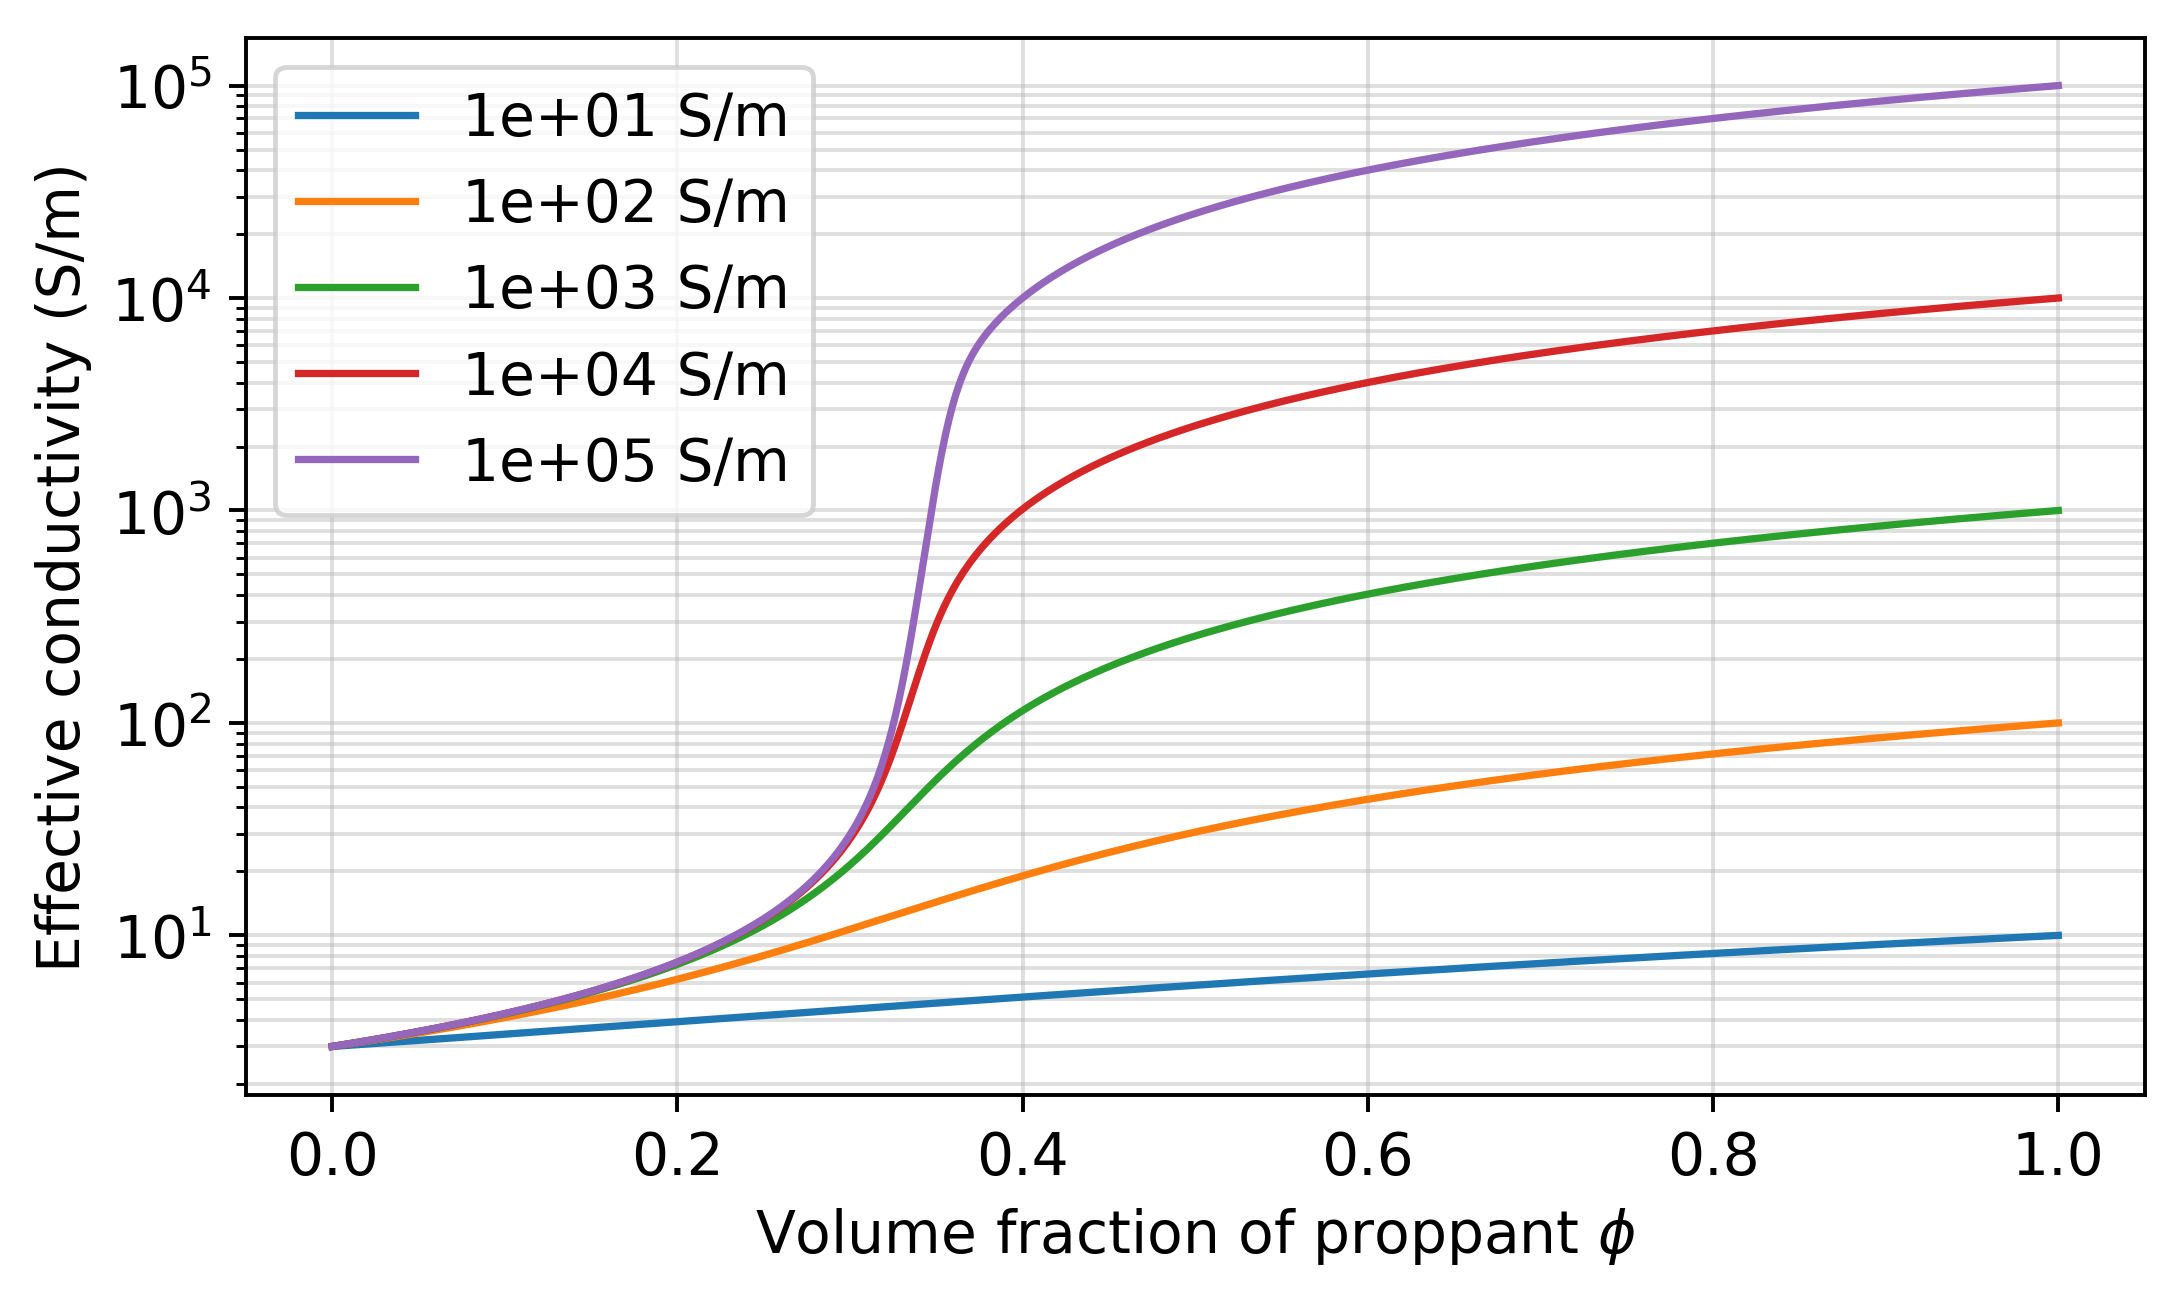
\includegraphics[width=0.6\textwidth]{figures/phys_prop_model/emt_spherical_particles.png}
    \end{center}
\caption{
    Effective conductivity of a proppant-fluid mixure for five different proppant
    conductivities, each indicated in the legend. Panel (a) shows the conductivity on a linear
    scale, and panel (b) uses a log-scale.
    The conductivity of the fluid is 3 S/m, similar to the conductivity of sea-water.
}
\label{fig:emt_spherical_particles}
\end{figure}


When the volume fraction of proppant is less than $1/3$, the conductivity of the fluid dominates is the dominant control on the resulting effective conductivity. Above a volume  fraction of $1/3$, the conductivity of the proppant is the primary contributor to the effective conductivity. The threshold between these behaviors is the \emph{percolation threshold}. Below it, the concentration of conductive material is low enough that it is quite likely disconnected, above $1/3$, the concentration is high enough to start forming connected, electrically conductive pathways, causing a large jump in the effective conductivity of the system. Although proppant typically composes 10\% to 20\% of the injected slurry, some of the injected fluid leaks off into the surrounding geologic formation leaving proppant concentration that can be 50\% in the fractures \cite{Novotny1977, Hoversten2015}.

The conductivity of the fluid also changes the resultant effective conductivity of the mixture. In Figure \ref{fig:emt_fluid}, we compare the effective conductivity for a mixture of conductive proppant (panel (a): $10^3$ S/m, panel (b): $10^4$ S/m) and four different fluid conductivities, ranging from 0.3 S/m to 300 S/m, as indicated in the legend. Although the conductivity of the fluid makes a significant difference at low proppant concentrations, above the percolation threshold of 33\%, the curves start to converge, particularly when the contrast between the conductivity of the proppant and the fluid exceeds 3 orders of magnitude. Thus, if the proppant can be made sufficiently conductive, its conductivity will be the controlling factor on the effective conductivity of the slurry that remains in the fractures.


\begin{figure}
    \begin{center}
    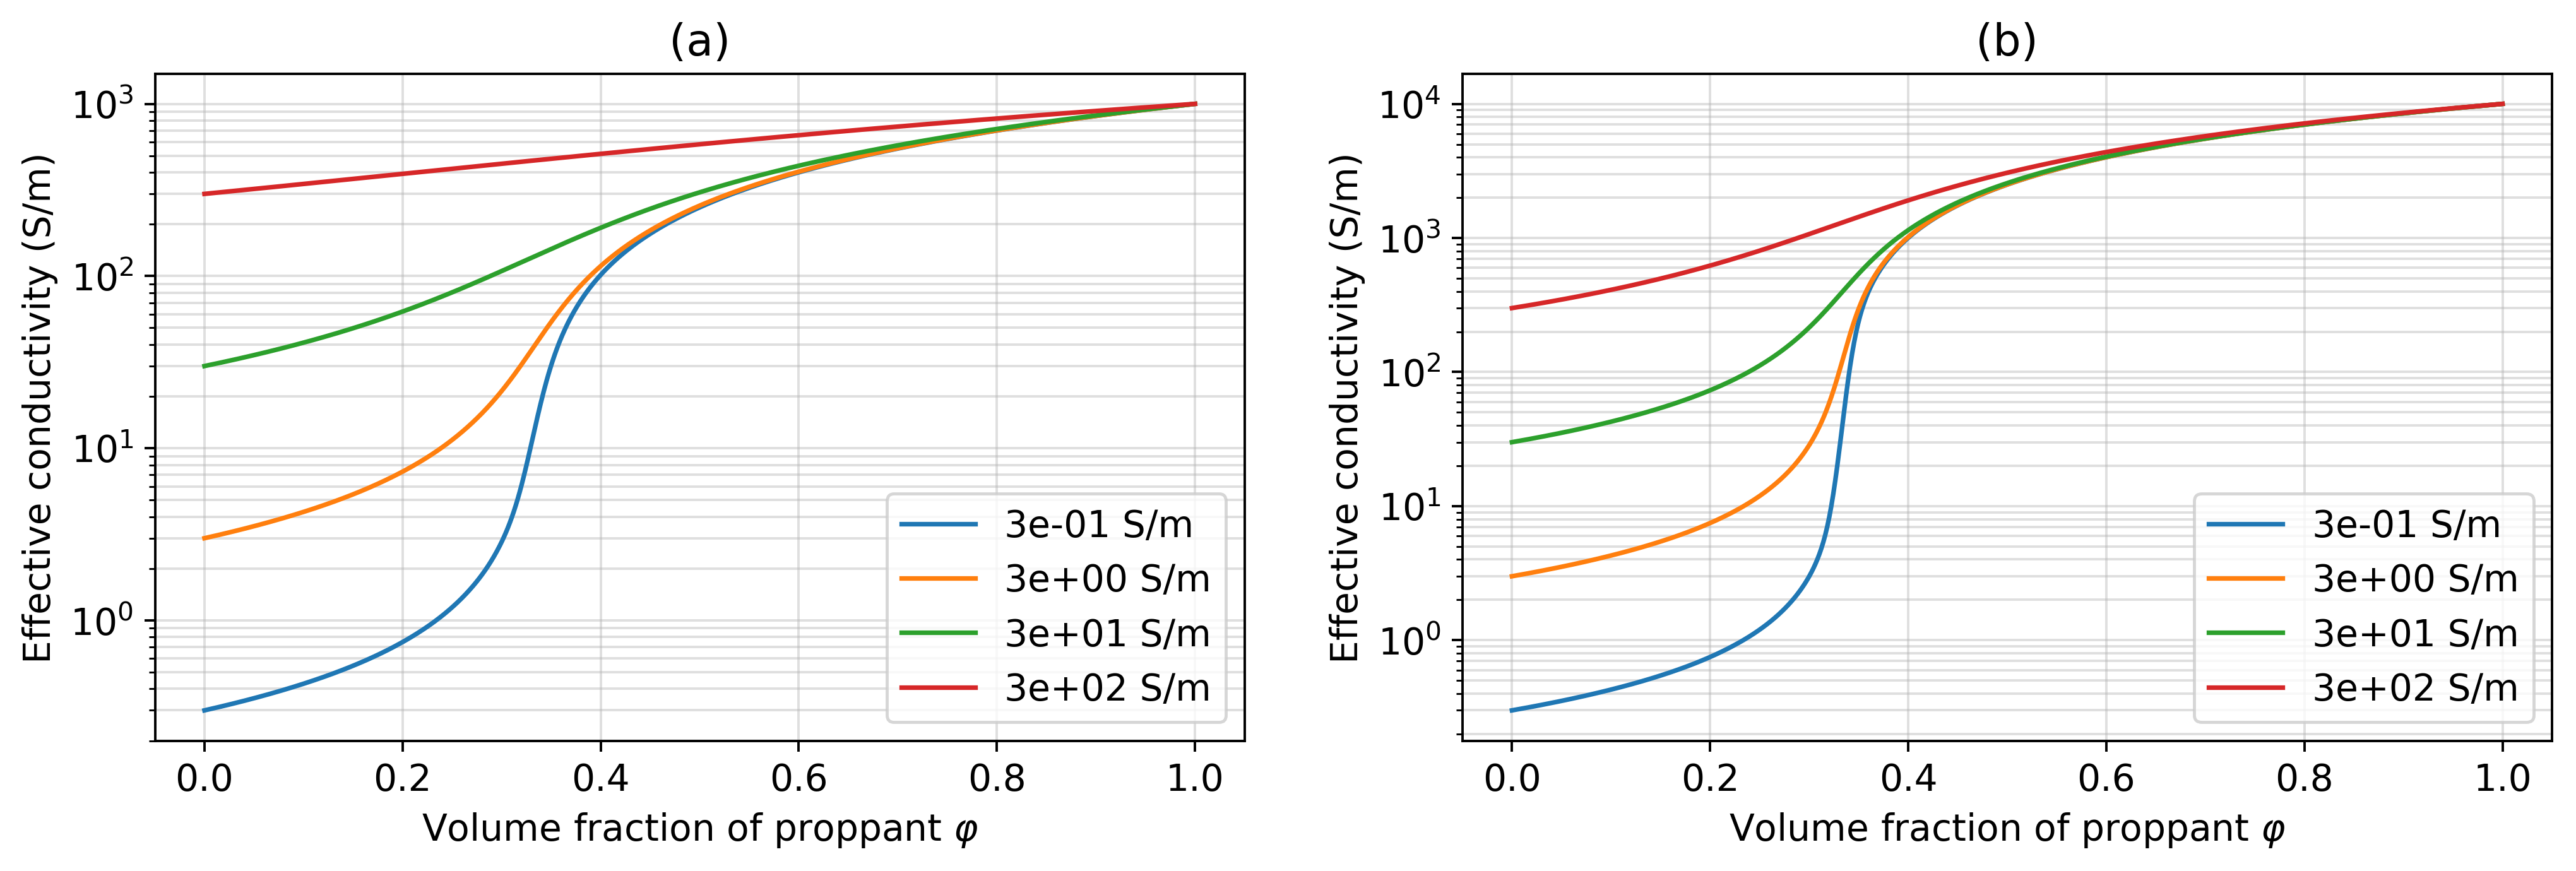
\includegraphics[width=\textwidth]{figures/phys_prop_model/emt_fluid.png}
    \end{center}
\caption{
    Impact of the conductivity of the fluid on the effective conductivity of a proppant-fluid mixture.
    Panels (a) and (c) show the effective conductivity for mixtures with a $10^3$ S/m proppant and panels
    (b) and (d) show the effective
    conductivity for mixtures with a $10^4$ S/m proppant. The conductivity of the fluid is indicated by the legend.
}
\label{fig:emt_fluid}
\end{figure}


The previous examples considered a 2-phase mixture in which all of the proppant was electrically conductive, however, depending on the setting and the cost to manufacture conductive proppant, it may be mixed in with conventional, resistive proppant. To examine this, we consider a proppant-fluid mixture composed of three materials, fluid ($3$ S/m), conventional, resistive proppant ($10^{-6}$ S/m) and conductive proppant ($10^5$ S/m). The effective conductivities of proppant-fluid mixtures for five different proppant blends, where the relative concentration of the conductive proppant is varied from 0\% to 100\% of the proppant phase, are shown in Figure \ref{fig:emt_3phase}. Again, we see the impacts of the percolation threshold; when the conductive proppant composes less than $1/3$ of the proppant pack, the effective conductivity is dominated by the resistive proppant. When the conductive proppant composes more than $1/3$ of the proppant pack, we see that with increasing proppant concentration, the effective conductivity of the mixture is dominated by the conductive proppant. However, the percolation threshold for each of these mixtures is different. This is because it is the role of the conductive proppant in the three-phase mixture, not the ratio of proppant to fluid, that determines when connected, electrically conductive pathways may be formed.


\begin{figure}
    \begin{center}
    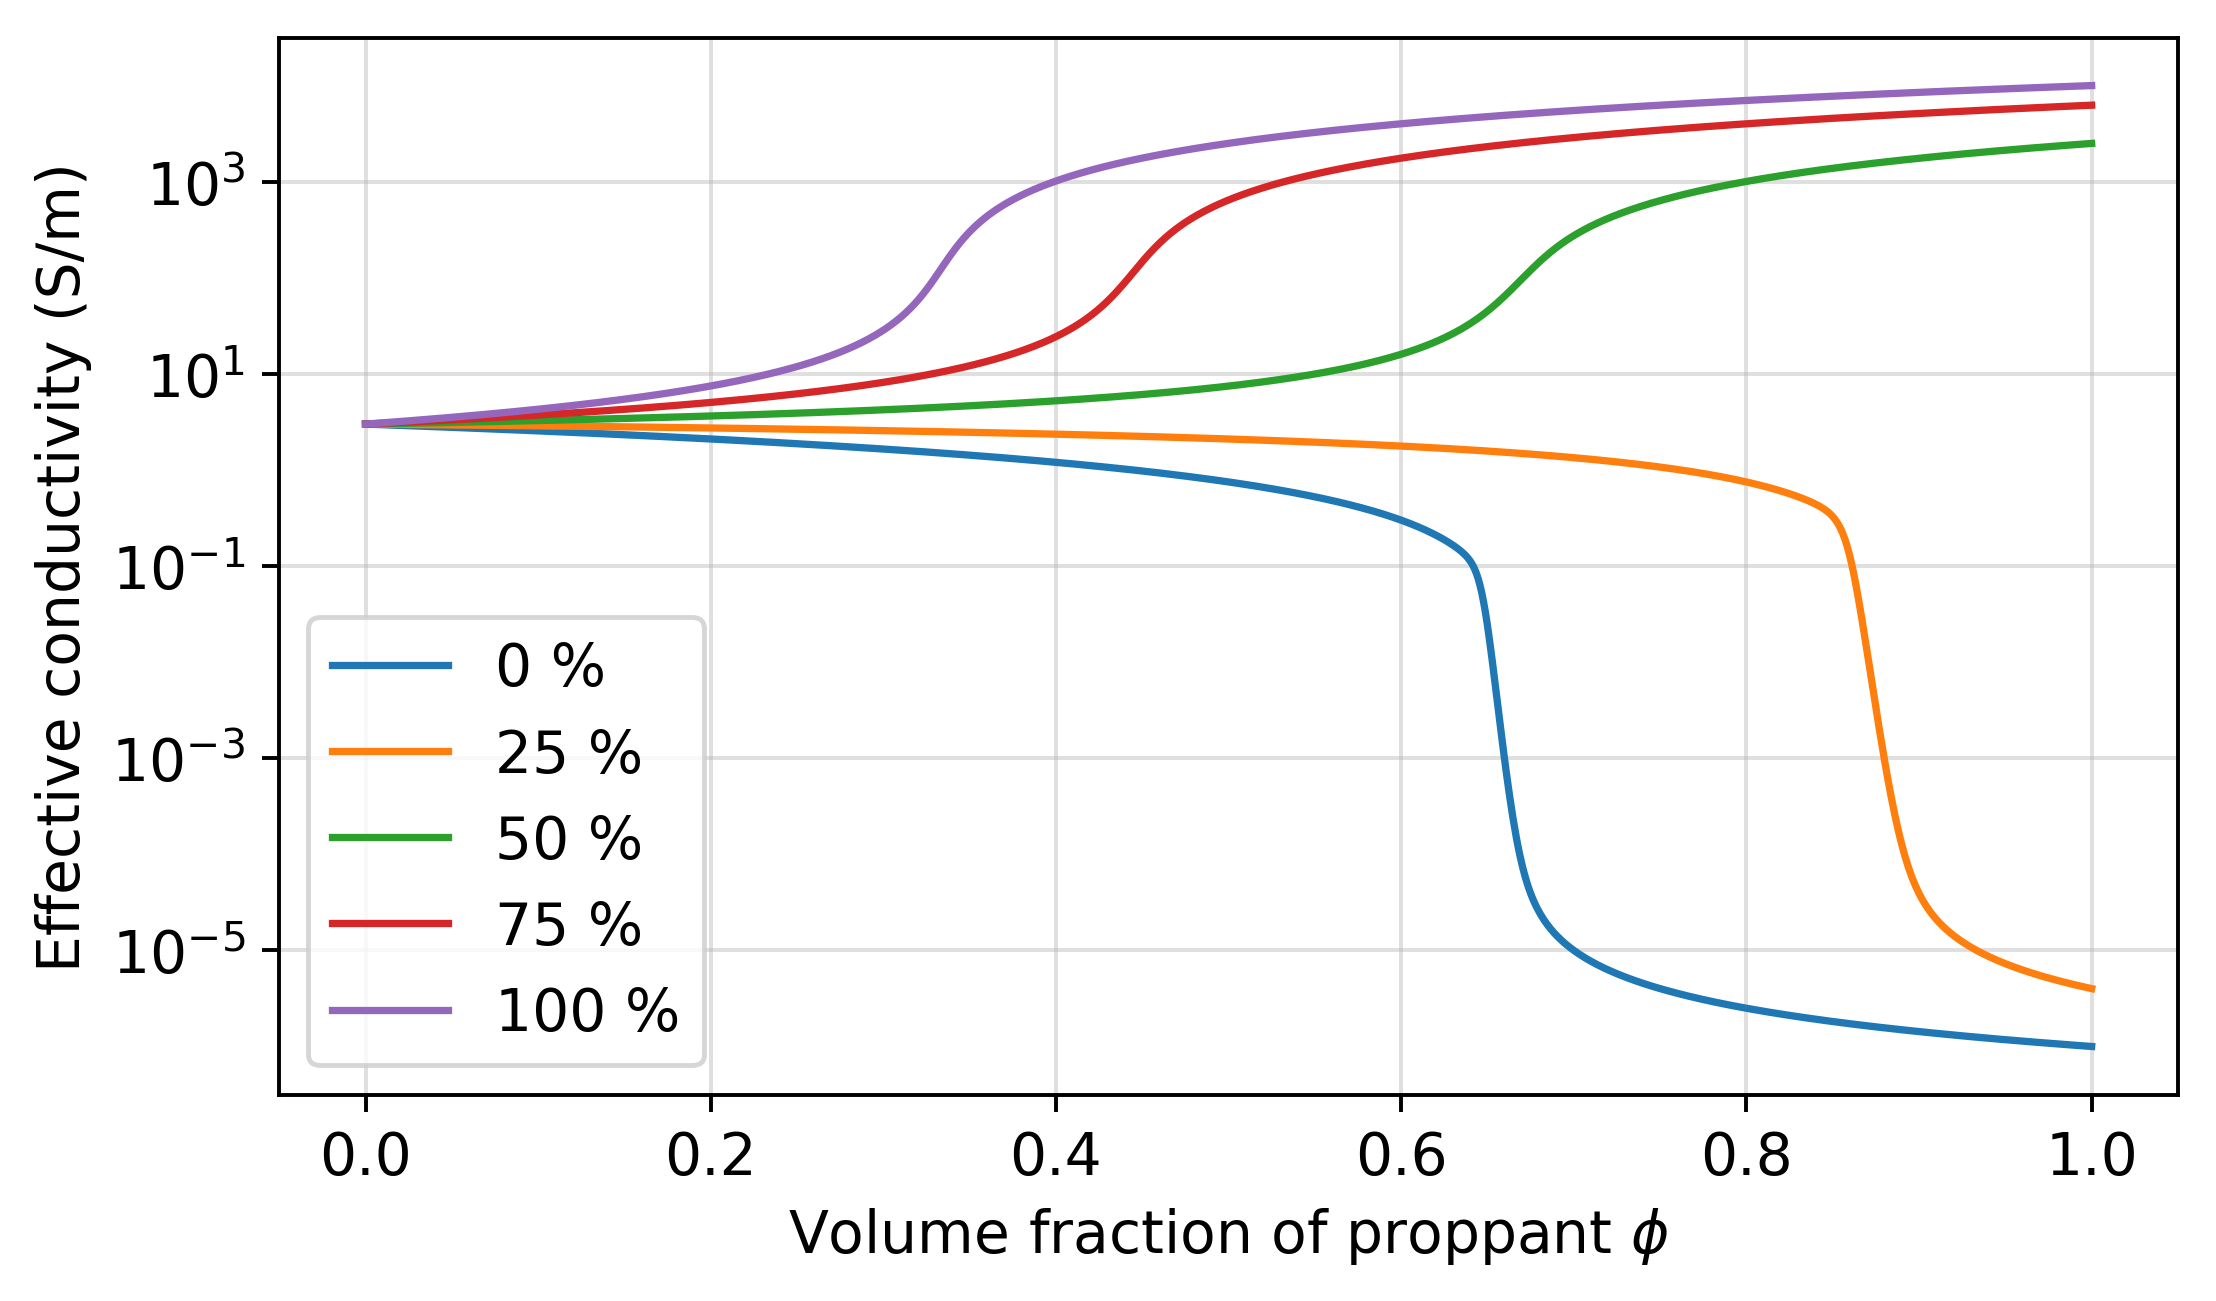
\includegraphics[width=0.6\textwidth]{figures/phys_prop_model/emt_3phase.png}
    \end{center}
\caption{
    Effective conductivity of a 3-phase proppant-fluid mixture consisting of
    resistive proppant ($10^{-6}$ S/m), conductive proppant ($10^5$ S/m) and saline
    fluid (3 S/m). The legend indicates the percentage of conductive proppant in the
    proppant mixture and the x-axis is the volume fraction of proppant in the
    proppant-fluid mixture.
}
\label{fig:emt_3phase}
\end{figure}


Another factor influencing the effective conductivity of a mixture is the shape of the materials. For the previous examples, the proppant was assumed to be composed of spherical particles. If elongated, conductive particles were included, we expect that connected, conductive pathways would form at lower concentrations. For instance, consider a 3 phase proppant mixture consisting of fluid (3 S/m), resistive, spherical proppant ($10^{-6}$ S/m), and elongated, electrically conductive proppant ($10^5$ S/m). Assume that the ratio of conductive to resistive proppant is 0.25 (below the percolation threshold for spherical particles). If the elongated particles (prolate spheroids) are randomly oriented, then the resulting effective conductivity is isotropic, meaning it is independent of the directions of the inducing field and resulting current. The conductivity predicted by effective medium theory for mixtures with five different aspect ratios is shown in figure \ref{fig:emt_3phase_aspect}. The aspect ratio of the conductive particles influences the concentration at which we observe percolation. The more elongated the particles, the lower the concentration at which percolation occurs.



\begin{figure}
    \begin{center}
    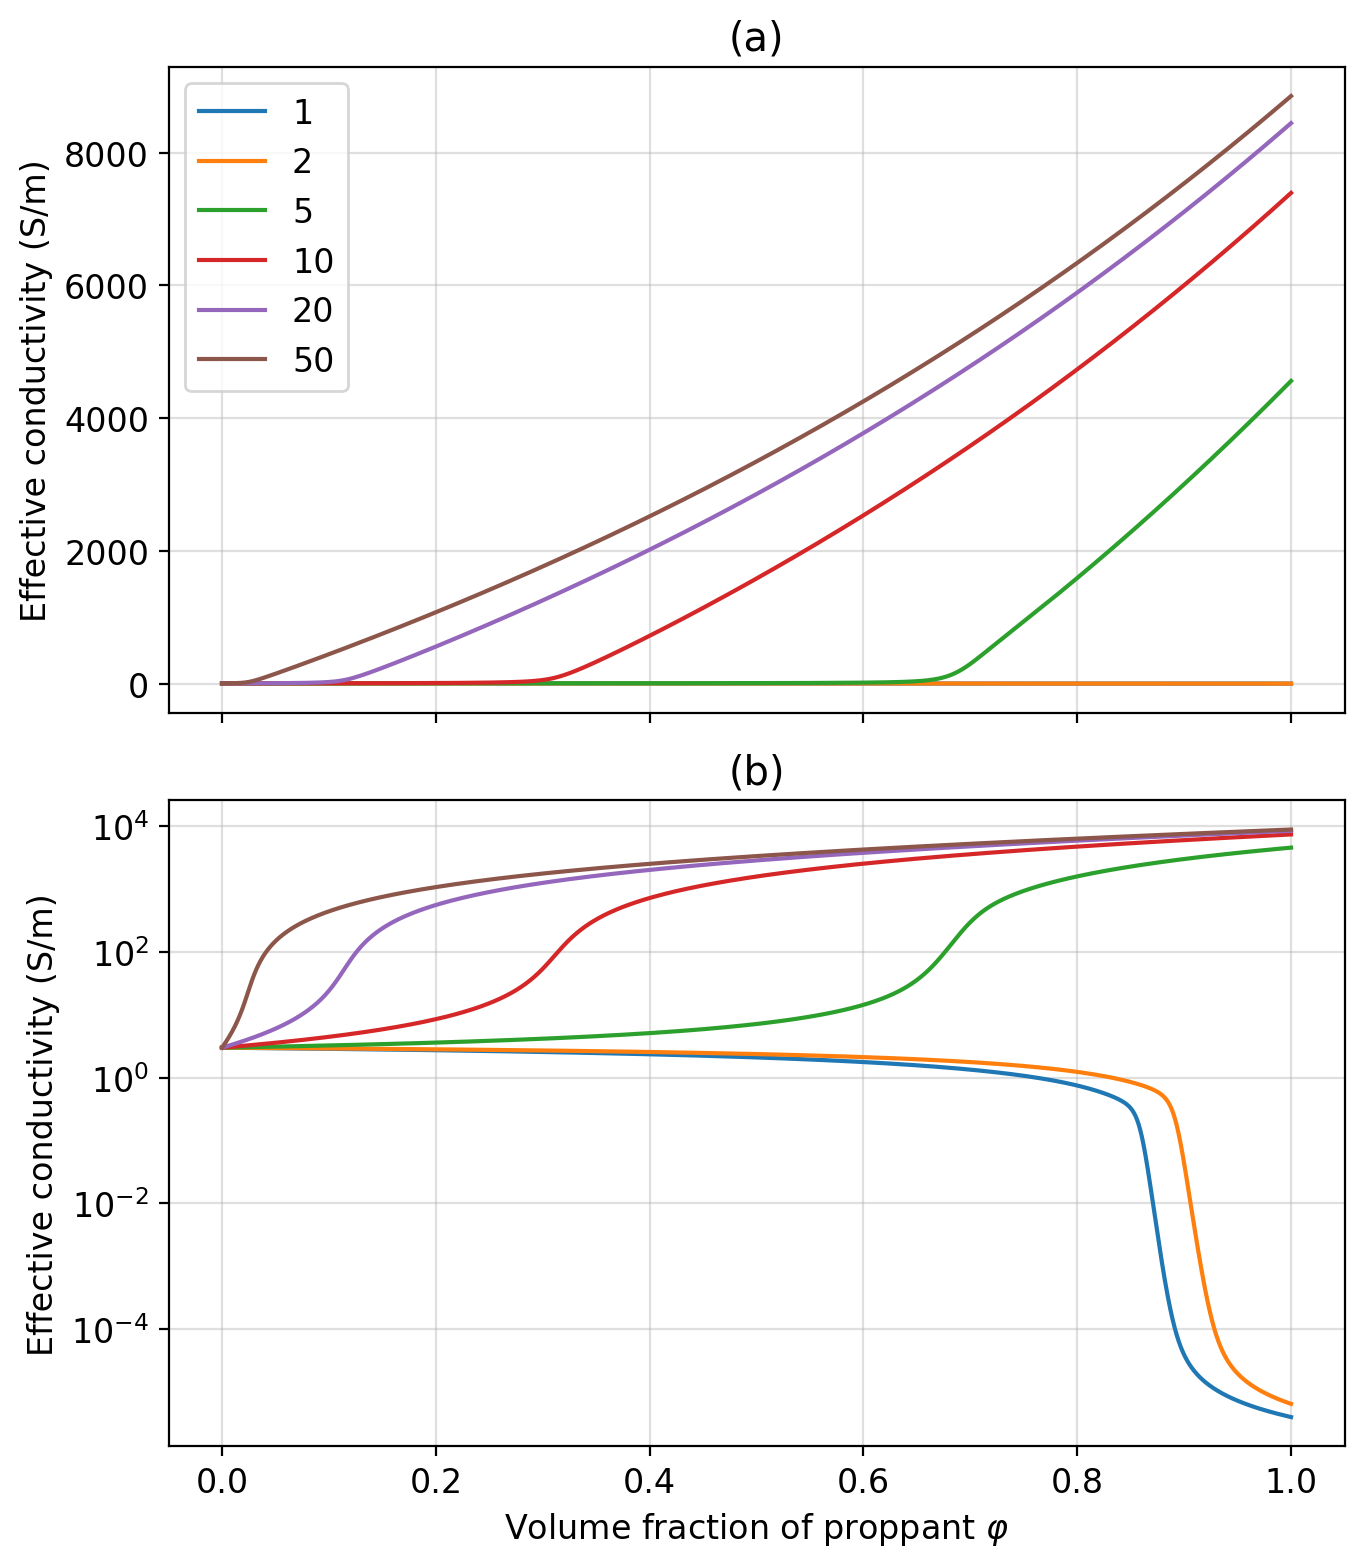
\includegraphics[width=0.6\textwidth]{figures/phys_prop_model/emt_3phase_aspect.png}
    \end{center}
\caption{
    Effective conductivity of a 3-phase proppant-fluid mixure consisting of
    resistive proppant ($10^{-6}$ S/m), conductive proppant ($10^5$ S/m) and saline
    fluid (3 S/m). The proppant mixture contains 25\% conductive proppant and
    75\% resistive proppant. The legend indicates the asppect ratio of the elongated
    conductive proppant filler (prolate spheroids).
}
\label{fig:emt_3phase_aspect}
\end{figure}


In summary, there are several approaches that can be taken to create an electrically conductive proppant-fluid mixture. Spherical proppant particles which are themselves electrically conductive or coated with a conductive material can comprise the entire proppant pack. If conductive proppant is mixed with a conventional, resistive sand or ceramic particles, then at least 1/3 of the proppant mixture needs to be comprised of electrically conductive particles to create a conductive mixture. This ratio can be reduced if elongated particles, such as metallic strips, are used in the proppant mixture.

\subsection{Step 2: Effective conductivity of fractured volume of rock}
The next step is to estimate the effective conductivity of a fractured volume of rock. We again employ self-consistent effective medium theory as described in section \ref{sect:emt_math} and consider the induced fractures to be composed of spheroidal cracks. Based on the analysis in the previous section, we consider a proppant-fluid mixture that has a conductivity of 2500 S/m. This could be achieved with spherical proppant particles having a conductivity of $10^4$ S/m in a 50/50 mixture with water of 3 S/m (see Figure \ref{fig:emt_spherical_particles}). Similar conductivities could be achieved with elongated particles mixed with conventional proppant as shown in Figure \ref{fig:emt_3phase_aspect}. Lab measurements conducted by \cite{Zhang2016} showed that a proppant-fluid mixture composed of petroleum coke particles and seawater which fills the pore-spaces reached a conductivity of $\sim 1000$ S/m at 37.6\% porosity. With further increase in confining pressure (thus reducing porosity and increasing the concentration of proppant), the observed conductivities of $3000 - 5000$ S/m. These results provide further confidence that conductivities $> 1000$ S/m for the mixture filling the hydraulic fractures are attainable.


For the following example, we will assume that the conductivity of the host-rock is 0.1 S/m. There are two scenarios we will consider, in the first, we assume the cracks are preferentially aligned, with the thin dimension of the oblate spheroid oriented along the y-axis. In this case, the recovered effective conductivity will be anisotropic, described by a diagonal matrix with entries $\sigma_x = \sigma_z \geq \sigma_y:$
\begin{equation}
    \Sigma^* = \left[
    \begin{array}{ccc}
    \sigma_x & & \\
    & \sigma_y & \\
    & & \sigma_z
    \end{array}
    \right]
    \label{eq:diagonal_sigma_e}
\end{equation}

Note that arbitrary, non-axes aligned, orientations can be considered; all that is required is that the depolarization tensor described in \ref{eq:emt_depolarization_tensor} is rotated to the desired orientation.

To estimate the effective conductivity of a fractured volume of rock, we must also specify the aspect ratio of the cracks. In estimating this, assume a fractal-like approximation, where the aspect ratio of the fracture is representative of the aspect ratio of the cracks that compose it. For example, if the fracture extends 50m laterally and has a width on the order of millimeters, then the aspect ratio is on the order of $10^{-5}$. In Figure \ref{fig:aligned_fractures}, we have plotted the diagonal elements of the effective conductivity for five different aspect ratios, indicated in the legend, as a function of the volume fraction of conductive fractures in the rock volume sampled. Panel (a) shows the full range from $0 \leq \phi \leq 1$ and panel (b) zooms in to lower concentrations ($0 \leq \phi \leq 0.01$) which are more representative of a fractured rock volume, on the scale that we will consider for numerical modelling (e.g. if 10 fractures, each with 3mm width intersect a 10m $\times$ 10m $\times$ 10m cell, then $\phi = 0.003$). In each of the plots, we have also included the upper and lower Wiener bounds (see equation 21.14 in \cite{Torquato2002}; originally attributed to \cite{Wiener1912}):
\begin{equation}
\begin{split}
\sigma_{\rm W}^{+} &= \sum_{j=0}^N \varphi_j \sigma_j \\
\sigma_{\rm W}^{-} &= \left(\sum_{j=0}^N \frac{\varphi_j}{\sigma_j}\right)^{-1}
\end{split}
\label{eq:wiener_bounds}
\end{equation}

in the black dashed lines; these can be understood as similar to parallel and series circuit approximations to the conductivity. In the black dash-dot lines are the upper and lower Hashin-Shtrikman bounds for 2-phase anisotropic media in the black dash-dot (see equations 21.25 and 21.26 in \cite{Torquato2002}, which is the anisotropic generalization of the isotropic bounds derived by \cite{Hashin1962}):
\begin{equation}
\begin{split}
\sigma_{\rm HS}^{+} &= \sigma_W^{+} \mathbf{I} + (\sigma_1 - \sigma_0)^2 \mathbf{\tilde{A}} \cdot
\left[\sigma_1\mathbf{I} + \frac{\sigma_1 - \sigma_0}{\varphi_0}\mathbf{\tilde{A}}\right]^{-1}\\
\sigma_{\rm HS}^{-} &= \sigma_W^{+} \mathbf{I} + (\sigma_1 - \sigma_0)^2 \mathbf{\tilde{A}} \cdot
\left[\sigma_0\mathbf{I} + \frac{\sigma_0 - \sigma_1}{\varphi_1}\mathbf{\tilde{A}}\right]^{-1}
\end{split}
\label{eq:hashin_shtrikman_bounds_anisotropic}
\end{equation}

For $\sigma_1 \geq \sigma_0$ and
\begin{equation}
\mathbf{\tilde{A}} = - \varphi_0\varphi_1\mathbf{A}_1
\label{eq:hashin_shtrikman_bounds_A}
\end{equation}

where $\mathbf{A}_1$ is the depolarization tensor for the ellipsoidal cracks given by equation \ref{eq:emt_depolarization_tensor}. For the bounds shown in the plot, the smallest aspect ratio, $10^{-5}$ was used to calculate the depolarization tensor. For the very significant aspect ratios used here, the Hashin-Shtrikman bounds are nearly identical to the Wiener bounds. Each component of the recovered effective conductivity should fall within these bounds.

\begin{figure}
    \begin{center}
    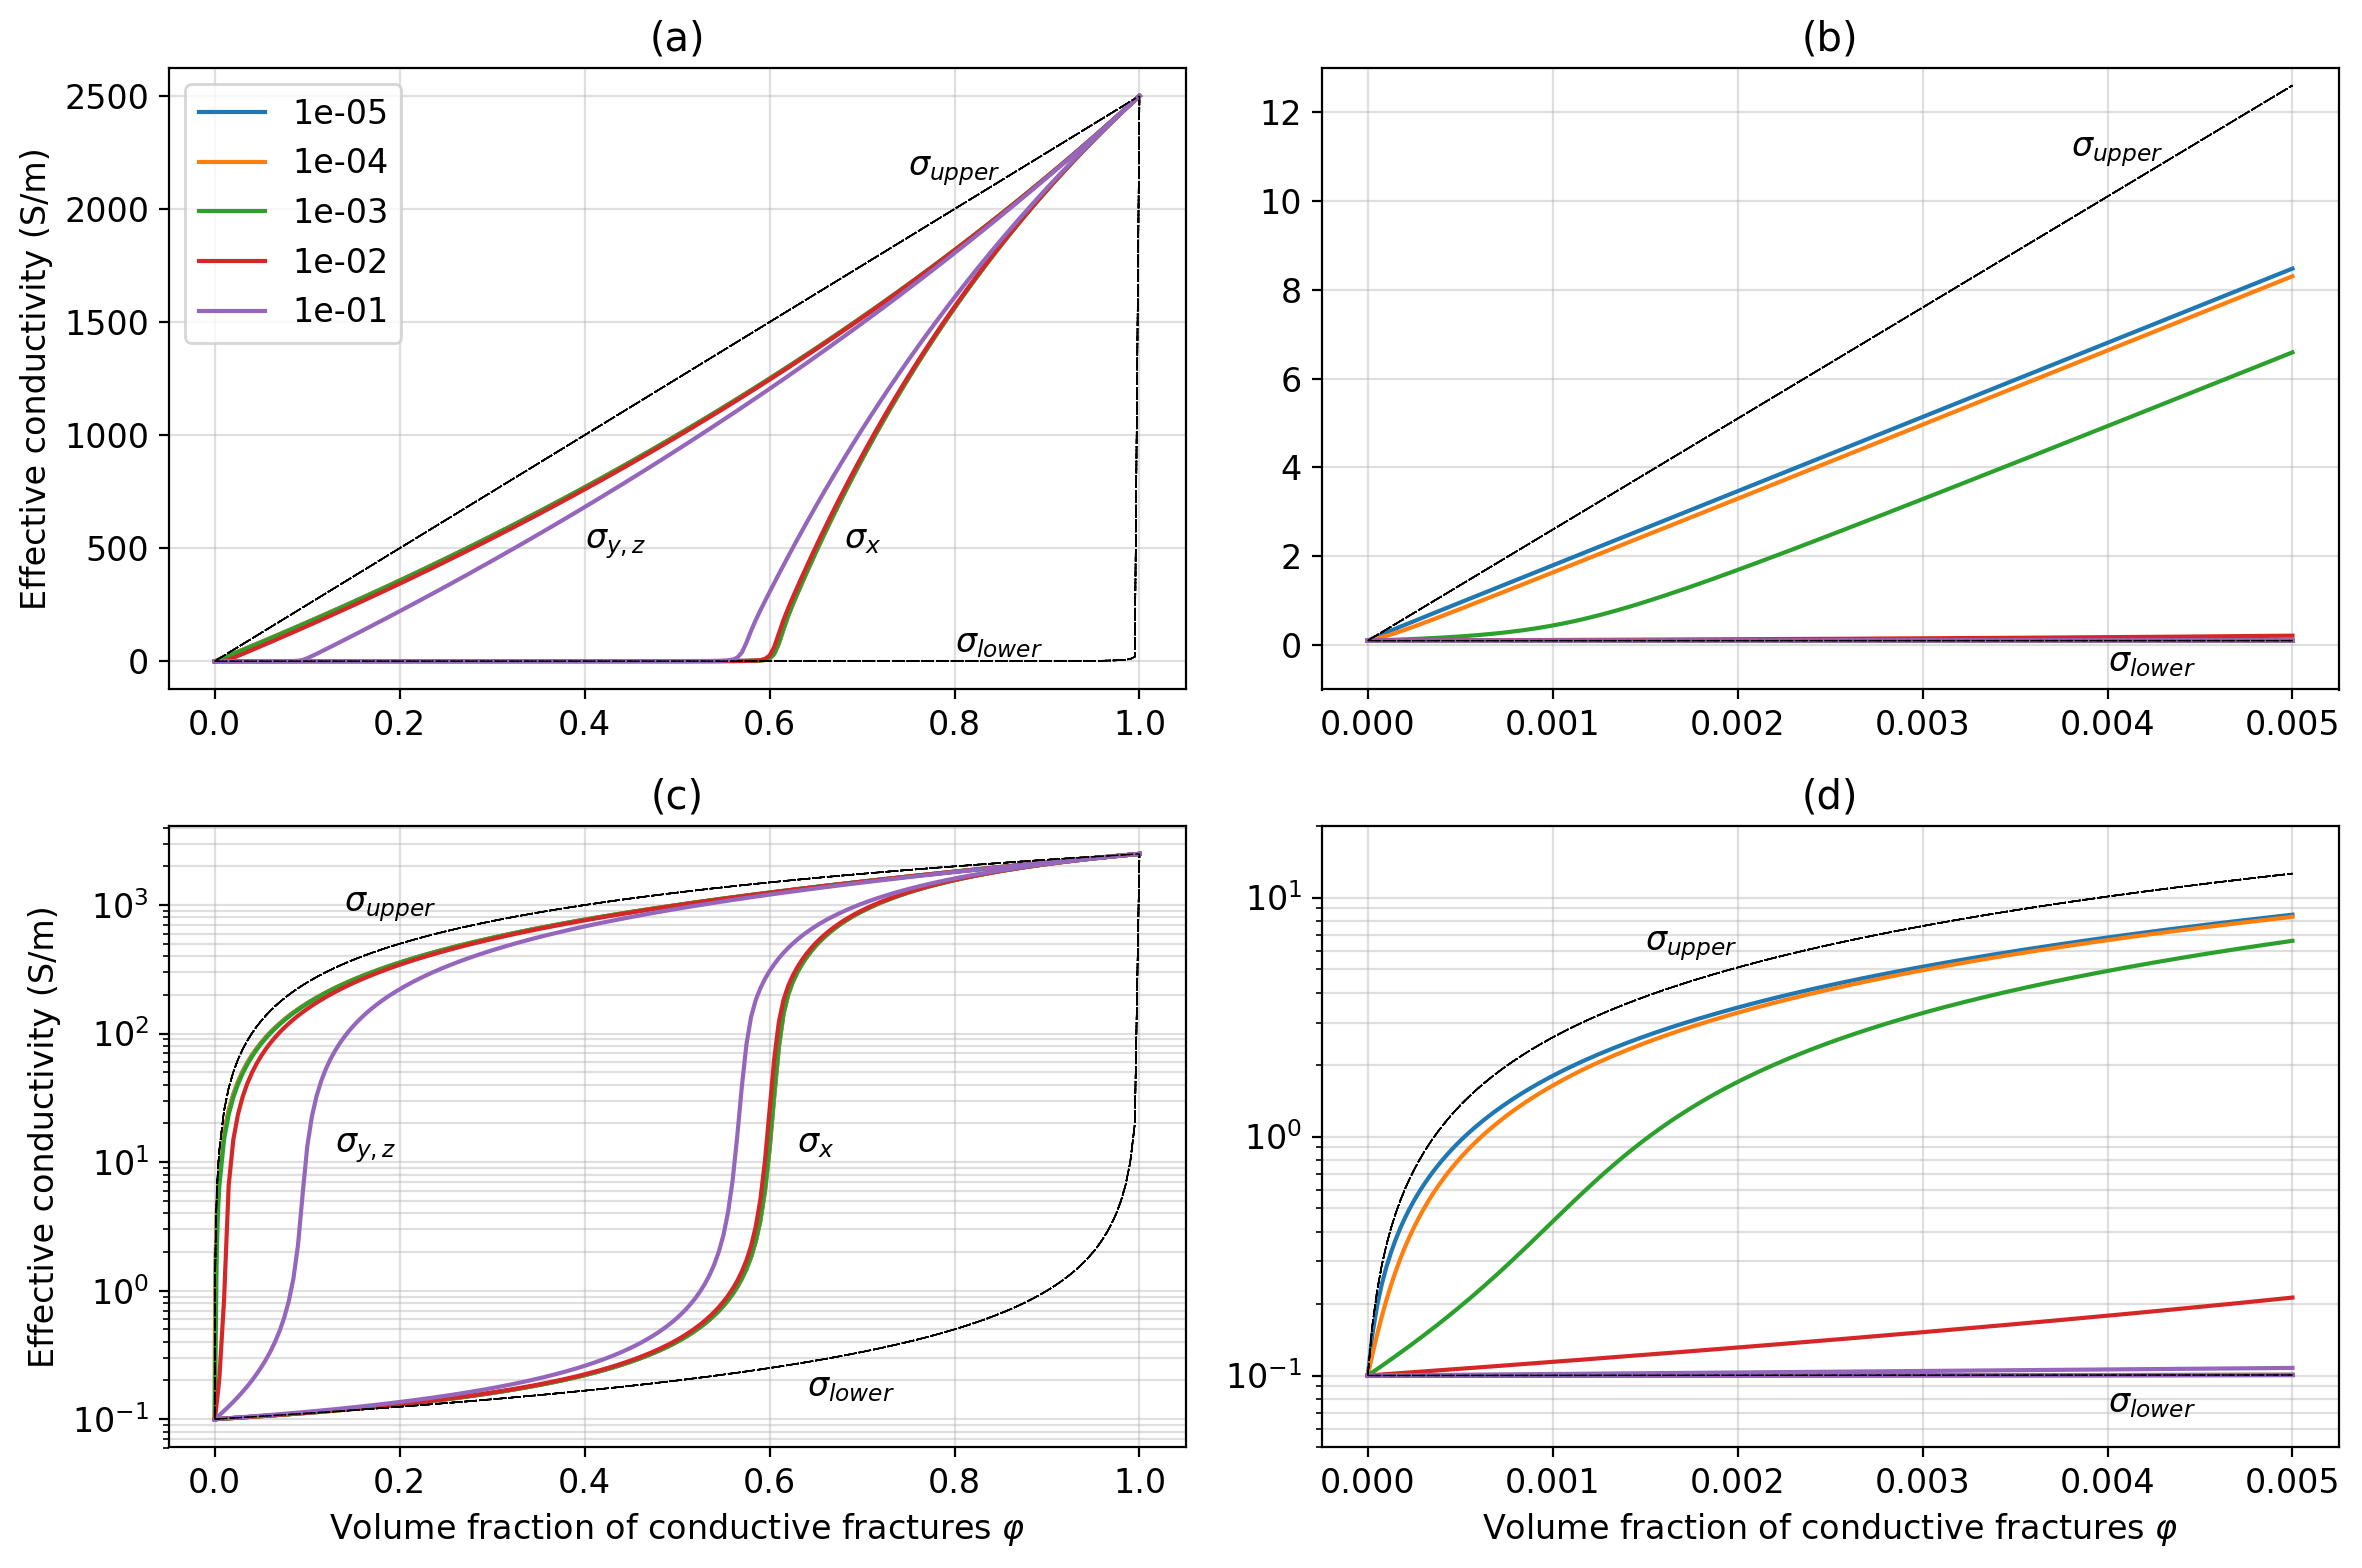
\includegraphics[width=\columnwidth]{figures/phys_prop_model/aligned_fractures.png}
    \end{center}
\caption{
    Effective, anisotropic conductivity for a fractured rock with spheroidal
    cracks whose normal is oriented along the x-axis for five different aspect ratios, indicated by the legend.
    The black dashed lines show the upper and lower
    Wiener Bounds, which are identical to the volume-weighted arithmetic and harmonic averages of the
    conductivity of the rock (0.1 S/m) and proppant-fluid mixture (2500 S/m). The black dash-dot lines
    are the anisotropic Hashin-Shtrikman upper and lower bounds computed using an aspect ratio of $10^{-5}$ in
    equation \ref{eq:hashin_shtrikman_bounds_anisotropic}. Note that the upper-bound coencides with $\sigma_{y, z}$ for small aspect ratios (e.g. the blue line).
    Panels (a) and (c) show the
    full range $0 \leq \varphi \leq 1$, and panels (b) and (d) zoom in to $0 \leq \varphi \leq 0.005$.
    Note that in (b), any curve that deviates from the lower bound is the $\sigma_{y, z}$ component;
    all $\sigma_x$ values lie on the lower bound for the concentration range shown.
}
\label{fig:aligned_fractures}
\end{figure}


For aspect ratios less than $10^{-3}$, we see very little distinction between the estimate of $\sigma_{x, z}$ and $\sigma_{y}$; the difference between the recovered effective conductivities for the aspect ratios of $10^{-4}$ and $10^{-5}$ is less than 1\% for all values of $\phi$. This indicates that for sufficiently thin cracks, the exact aspect ratio is not critical for estimating a representative conductivity of the fractured rock.

At the concentrations we expect to be observing in a hydraulic fracturing scenario (Figure \ref{fig:aligned_fractures}b), we see that the effective conductivity along the normal of the fractures coincides with the lower bounds and remains nearly identical to the conductivity of the host rock for all aspect ratios shown, as may be expected. For the components of the conductivity along the cracks ($\sigma_{x, z}$), the effective conductivity mimics the behavior of the upper bounds. These components of the conductivity are similar to the behavior expected from a parallel-circuit approximation.

For settings where planar fractures are expected, an single orientation of the inclusions produces similar behavior to what would be expected if we performed simple series-and-parallel circuit approximations to the components perpendicular to and along the fracture. However, if more complex fracture networks are expected, it may be more appropriate to assume the cracks are randomly oriented. In this case, an isotropic conductivity describes the fractured volume of rock. Using the same aspect ratios shown in Figure \ref{fig:aligned_fractures} above, we compute the isotropic effective conductivity as a function volume fraction of fractures in Figure \ref{fig:random_fractures}. For reference, the conductivity along the fractures, $\sigma_{x, z}$ from Figure \ref{fig:aligned_fractures}, is plotted in semi-transparent lines. As in the previous Figure, panel (a) shows the full range from $0 \leq \phi \leq 1$ and panel (b) zooms in to lower concentrations: $0 \leq \phi \leq 0.01$.

\begin{figure}
    \begin{center}
    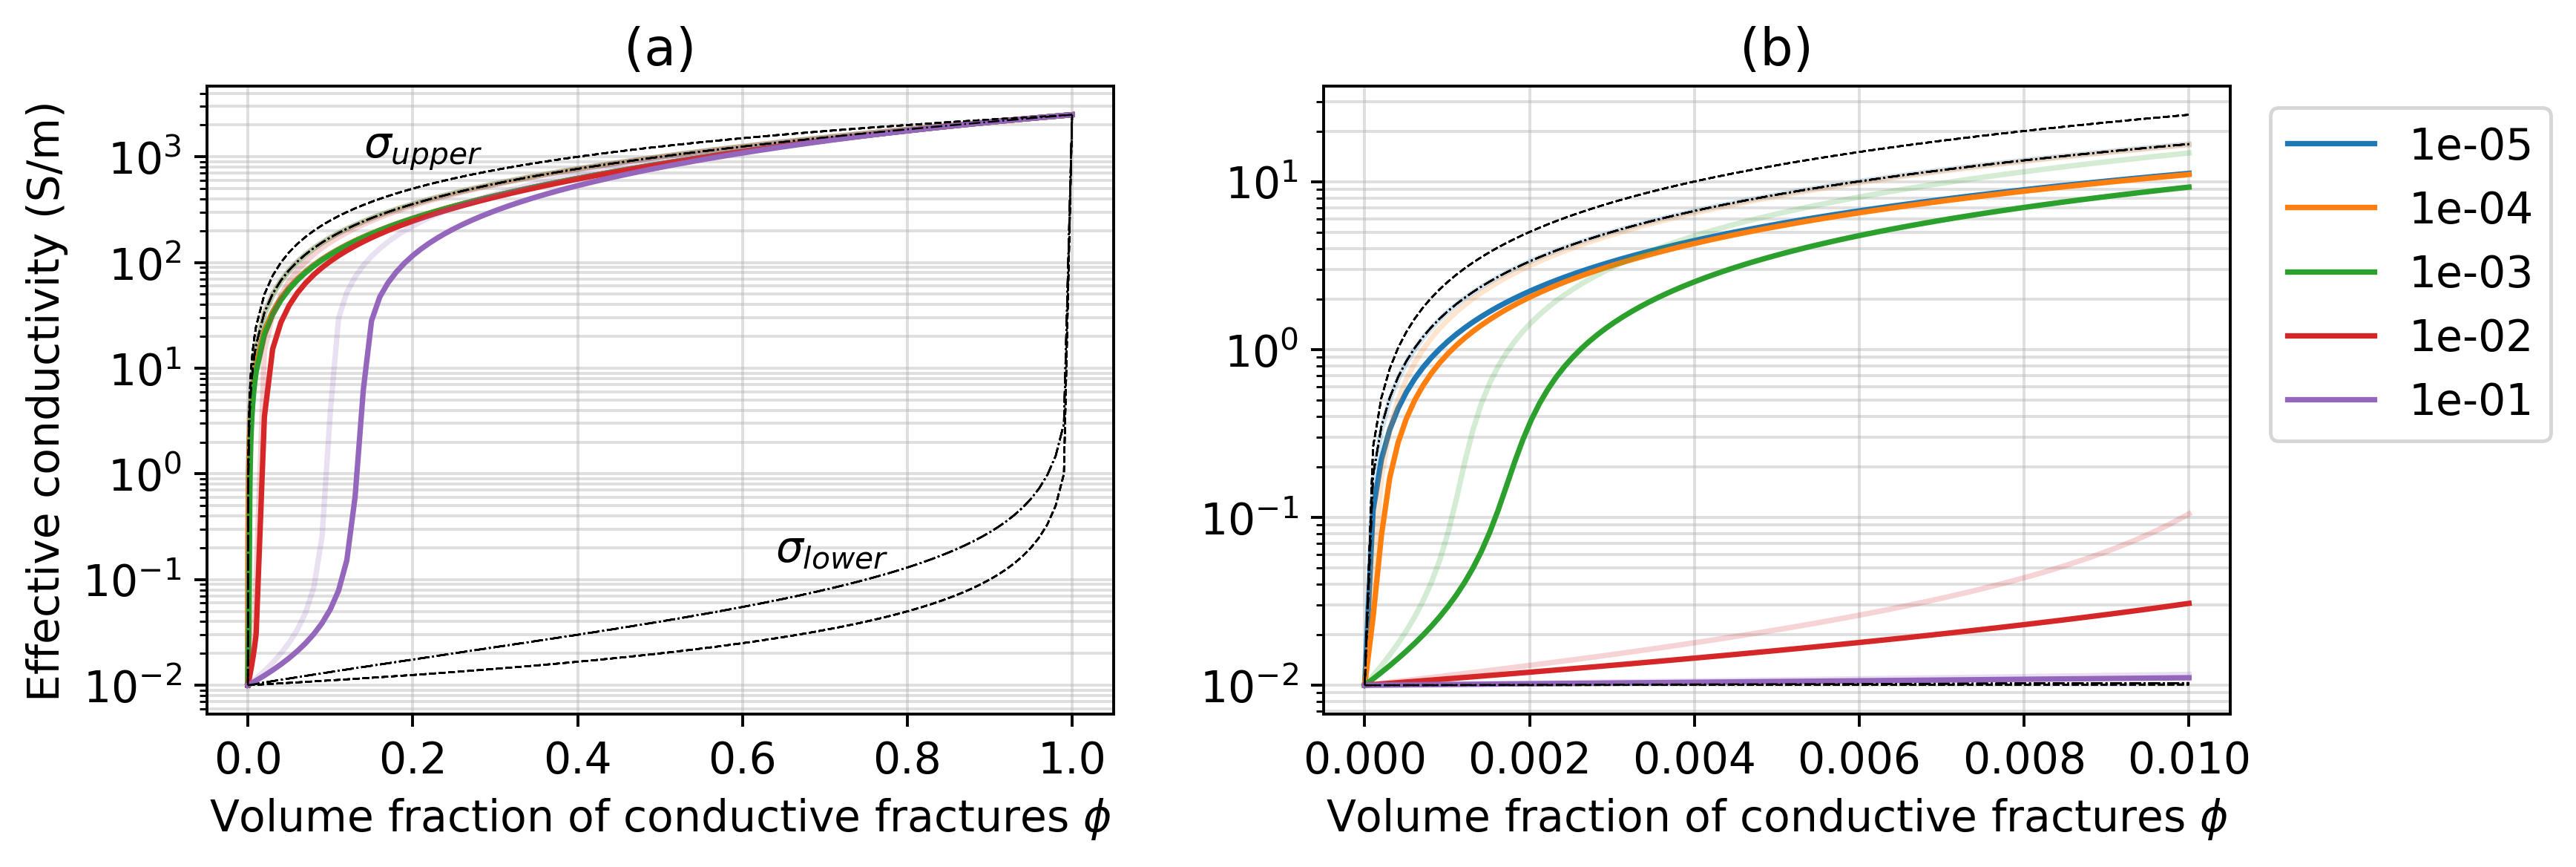
\includegraphics[width=\columnwidth]{figures/phys_prop_model/random_fractures.png}
    \end{center}
\caption{
    Effective, isotropic conductivity for a fractured rock with randomly oriented spheroidal
    cracks for five different aspect ratios, indicated by the legend. The black dashed lines show the upper and lower
    Wiener Bounds, which are identical the volume-weighted arithmetic and harmonic averages of the
    conductivity of the rock (0.1 S/m) and proppant-fluid mixture (2500 S/m).The black dash-dot lines
    are the isotropic Hashin-Shtrikman upper and lower bounds.
    The semi-transparent dotted lines show $\sigma_{y, z}$ from Figure \ref{fig:aligned_fractures}
    Panels (a) and (c) shows the
    full range $0 \leq \varphi \leq 1$, and panels (b) and (d) zooms in to $0 \leq \varphi \leq 0.01$.
}
\label{fig:random_fractures}
\end{figure}


Again, we see that for aspect ratios smaller than $10^{-3}$ there is little difference between the estimated effective conductivity of the fractured rock volume. The estimate of the effective conductivity largely follows the behavior of the upper bounds, while the magnitude of the effective conductivity is slightly reduced as compared to the component of the conductivity along the fractures in the anisotropic case. If we consider a $10m \times 10m \times 10m$ computational cell with fractures having an aspect ratio of $10^{-5}$ and composing 0.3\% of the total volume (e.g. 10 fractures, each with 3mm width), we obtain $\sigma_x = \sigma_z = 5.2$ S/m, $\sigma_y = 0.1$ S/m for the case where the cracks are preferentially aligned while for the case where the cracks are randomly oriented, we obtain $\sigma^* = 3.5$ S/m.

Due to the large contrast between the conductive fractures and the host rock, the conductivity of the background has marginal effect on $\sigma_{x, z}$ in the anisotropic example or on $\sigma^*$. If we consider the example with $\phi = 0.003$, as before, and instead use a background conductivity of 0.01 S/m, the effective anisotropic conductivity is $\sigma_x = \sigma_z = 5.1$ S/m, $\sigma_y = 0.01$ S/m and for the isotropic case $\sigma^* = 3.4$ S/m. However, if the background is made more conductive and the contrast between the conductive fractures and the host reduced, we do see some impact. Setting the background to 1 S/m for this same example, we obtain $\sigma_x = \sigma_z = 6.4$ S/m, $\sigma_y = 1$ S/m for the anisotropic case and $\sigma^* = 4.7$ S/m for the isotropic case.


\subsection{Summary}
To construct an approximate conductivity model of a fractured volume of rock, we use a two step process: first, we estimate the effective conductivity of a mixture of proppant and fluid that fills the fractures and second, we estimate the effective conductivity of a fractured volume of rock.

In the section that follows, we will compare numerical simulations of a cross-well electromagnetic survey for both anisotropic and isotropic conductivity models of a fractured volume of rock, representing planar and complex fracture networks, respectively.


